\section{Measurement Results and Evaluation}

\subsection{Errors and countrate}
The number $N$ of measurement events of a channel of the MCAs is Poisson distributed. Hence the error $s_N$  of $N$ events is:
\begin{equation}
  s_N = \sqrt{N}
\end{equation}

Not all meassurements were done in the same amount of time, so we decided to normalize all measured data with the elapsed time $t$ to a 
countrate $n$. Consequently the error changes, too:
\begin{equation}
    n = \frac{N}{t}, \qquad s_n = \frac{s_N}{t}
\end{equation}

\subsection{Energy resolution}

\subsection{Energy calibration}
\begin{figure}[H]
\begin{center}
  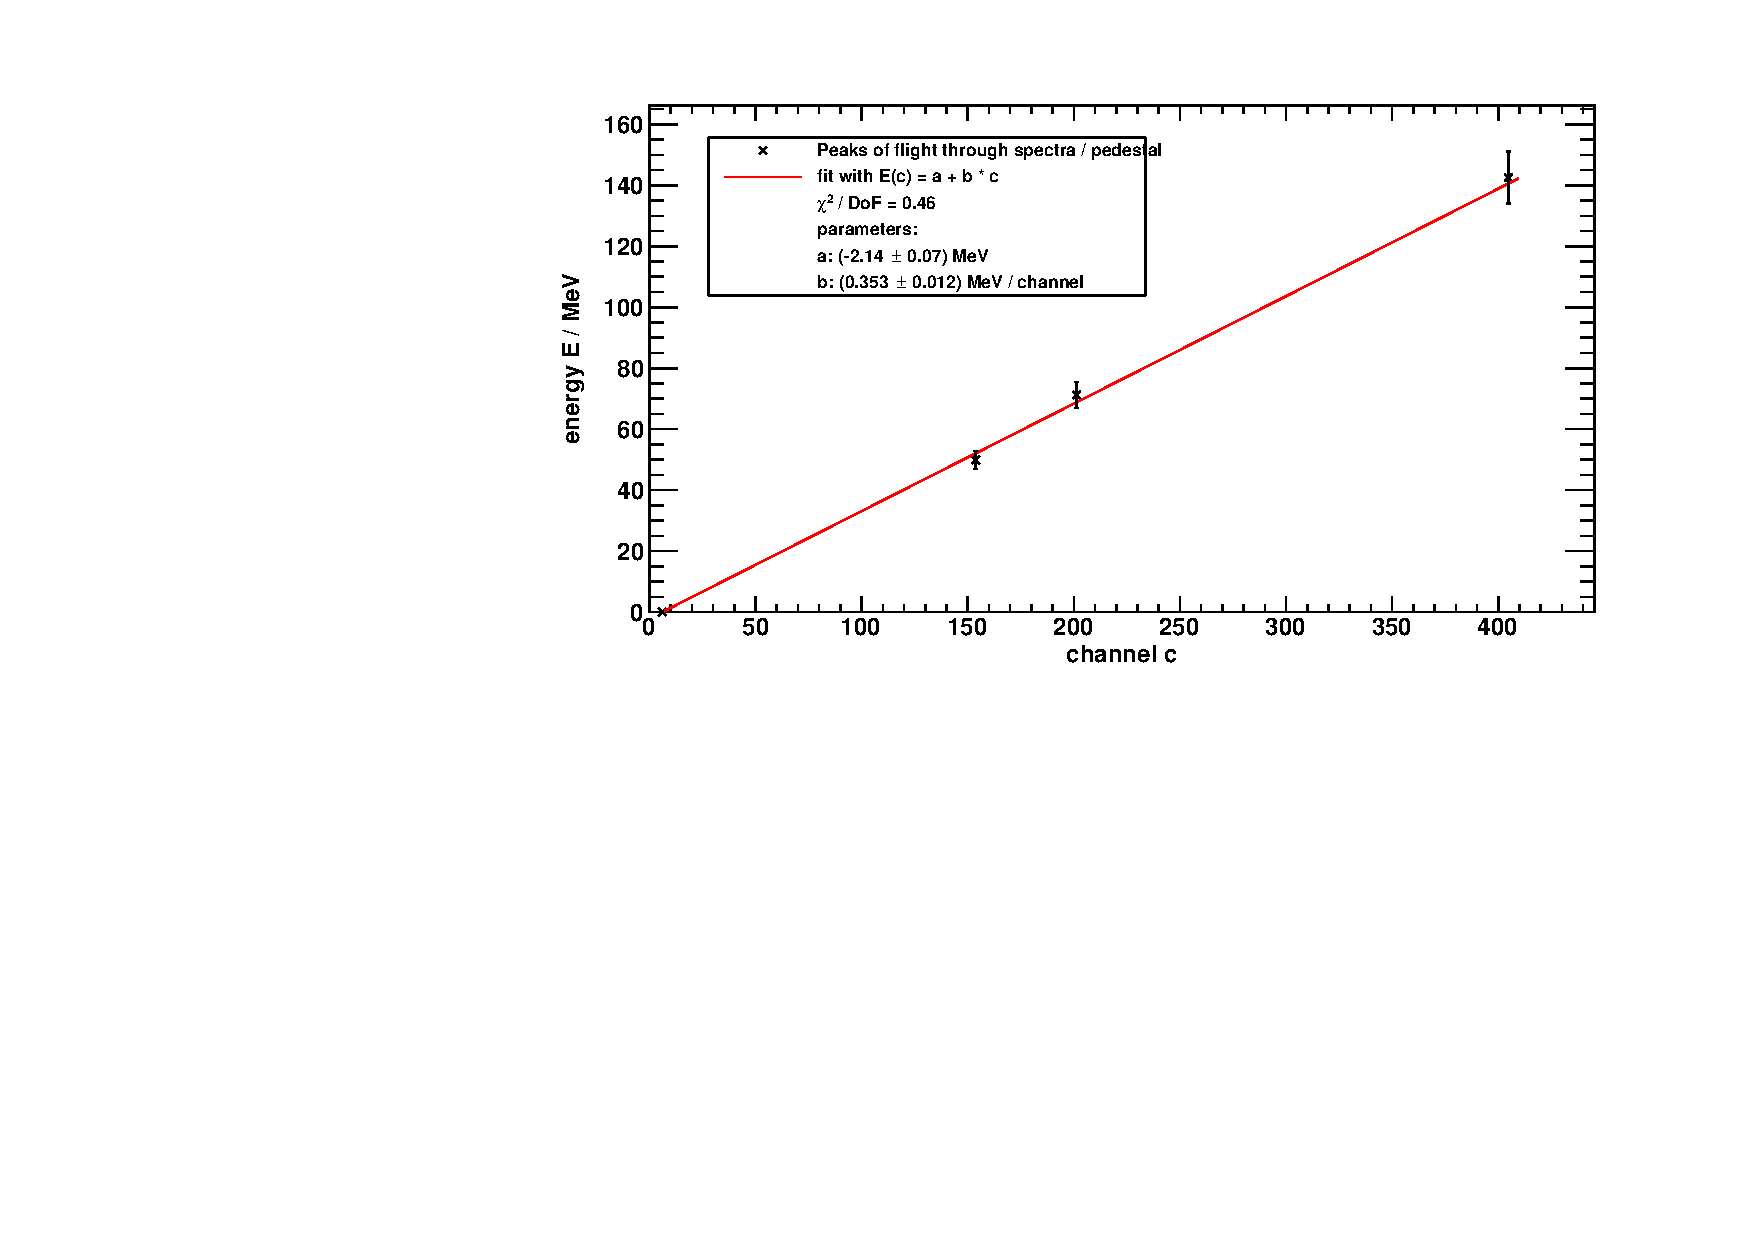
\includegraphics[width=\textwidth]{../img/energyCalibration.pdf}
  \caption{Energy calibration.}
  \label{img:energycalibration}
\end{center}
\end{figure}

\subsection{Time calibration}
\begin{figure}[H]
\begin{center}
  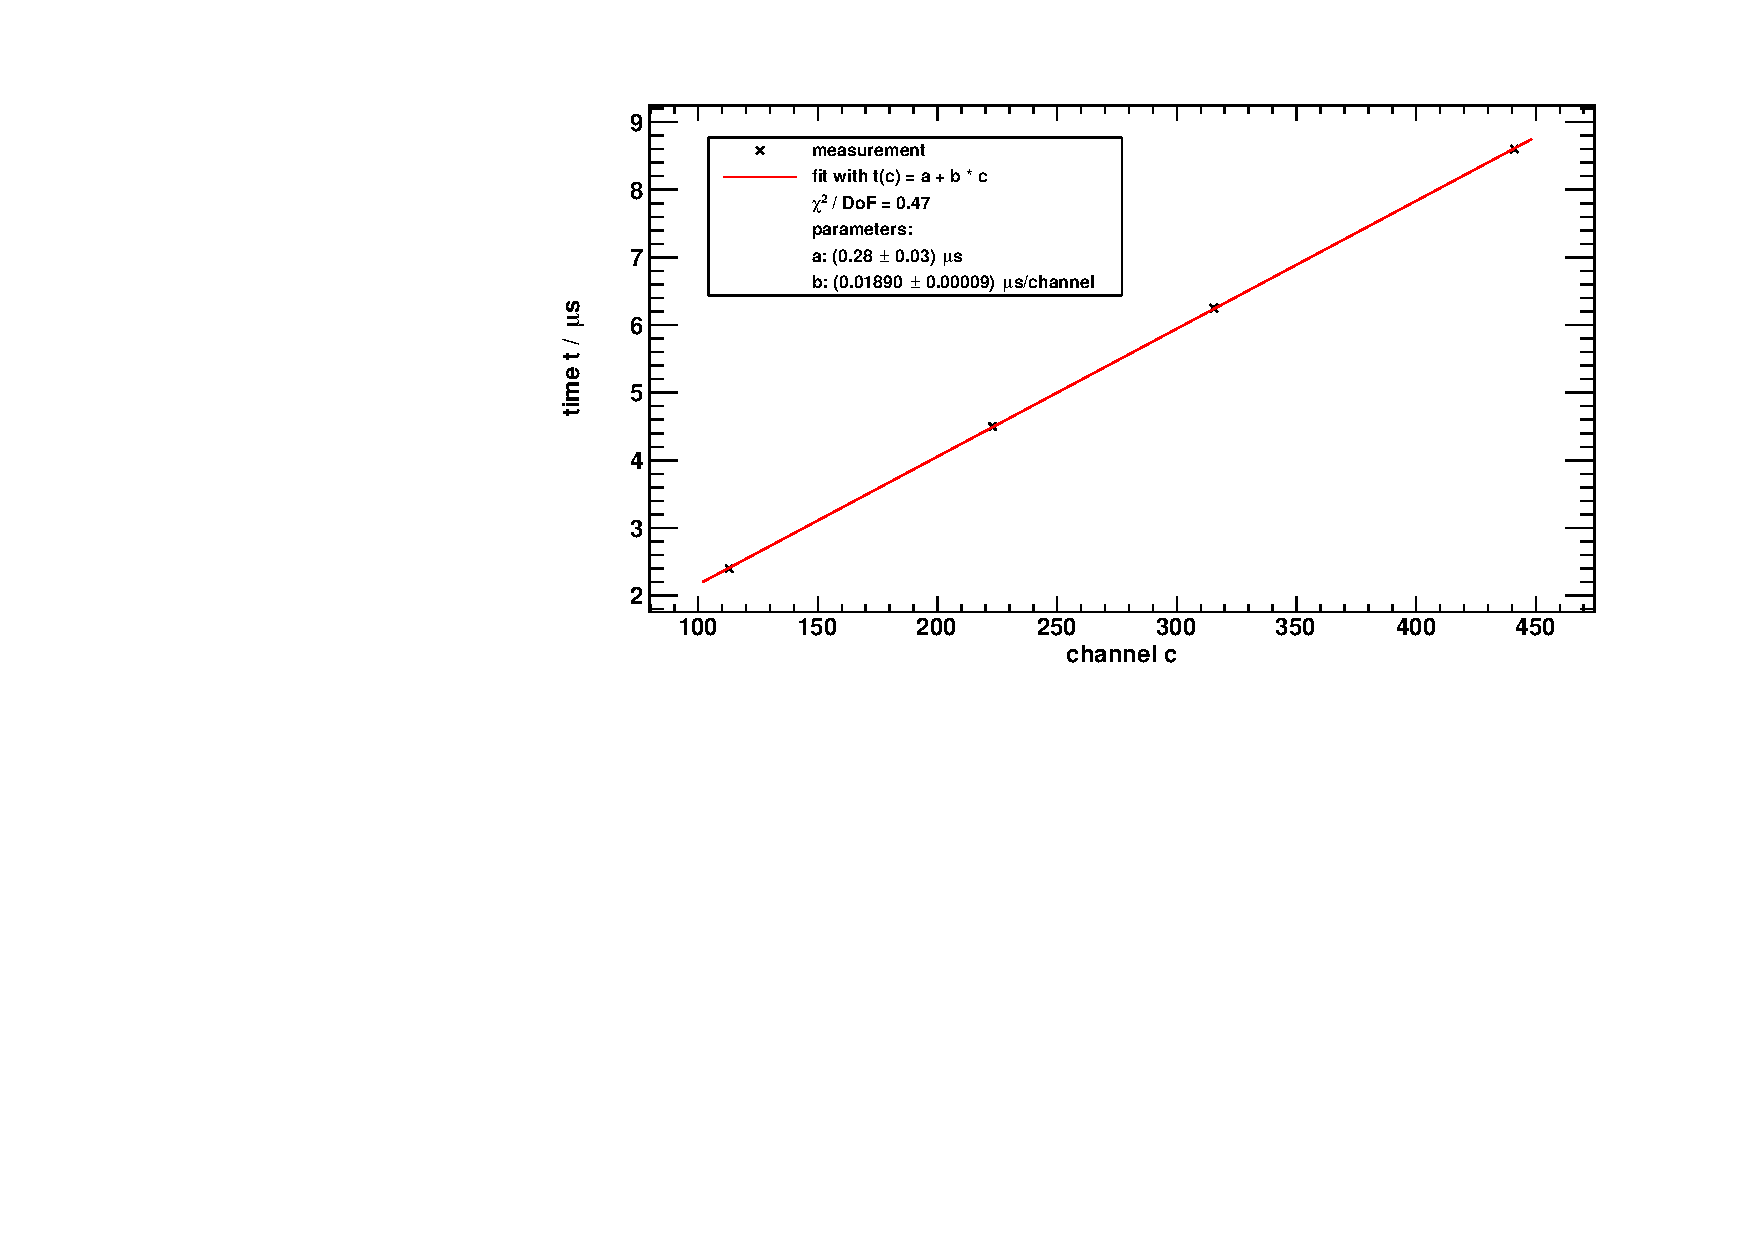
\includegraphics[width=\textwidth]{../img/timeCalibration.pdf}
  \caption{Time Calibration.}
  \label{img:timecalibration}
\end{center}
\end{figure}

\begin{equation}
\label{eq:tcalibration}
    t = a + b \cdot c, \qquad s_t = \sqrt{s_a^2 + \left(x \cdot s_b \right)^2 + 2 \cdot x \cdot \cov(a,b)}
\end{equation}

\subsection{Underground}

\subsection{$\beta$-spectrum}

\subsection{Decay time}
To calculate the decay time $\tau$ of $\mu$ the channels are converted to a time with \autoref{eq:tcalibration}. 
The so obtained datapoints get fitted with an exponential function:
\begin{equation}
    
\end{equation}